\chapter{Introduction}
\label{chap:ch1}

\section{About}
\label{chap:ch1sec1}

\par Introducere: obiectivele lucrării și descrierea succintă a capitolelor, prezentarea temei, prezentarea contribuției proprii, respectiv a rezultatelor originale și menționarea (dacă este cazul) a sesiunii de comunicări unde a fost prezentată sau a revistei unde a fost publicată.

\section{Related work}
\label{chap:ch1sec2}


\indent\par Informatii si citare carte \cite{Sommerville2010}.

Informații și citare articol publicat la conferință (in proceedings) \cite{Narayan2012}.

Informații și citare articol publicat în revista \cite{Robbes2015}.

Informații și citare articol publicat tip masterthesis  \cite{mastersthesis1993}.

Informații și citare articol publicat tip phdthesis \cite{phdthesis1993}.

Informații și citare articol ca resursă Internet  \cite{kinaSUR}.

Inserarea și Referirea unei figuri \ref{FigCBSD}.

\begin{figure}[htbp]
	\centering
		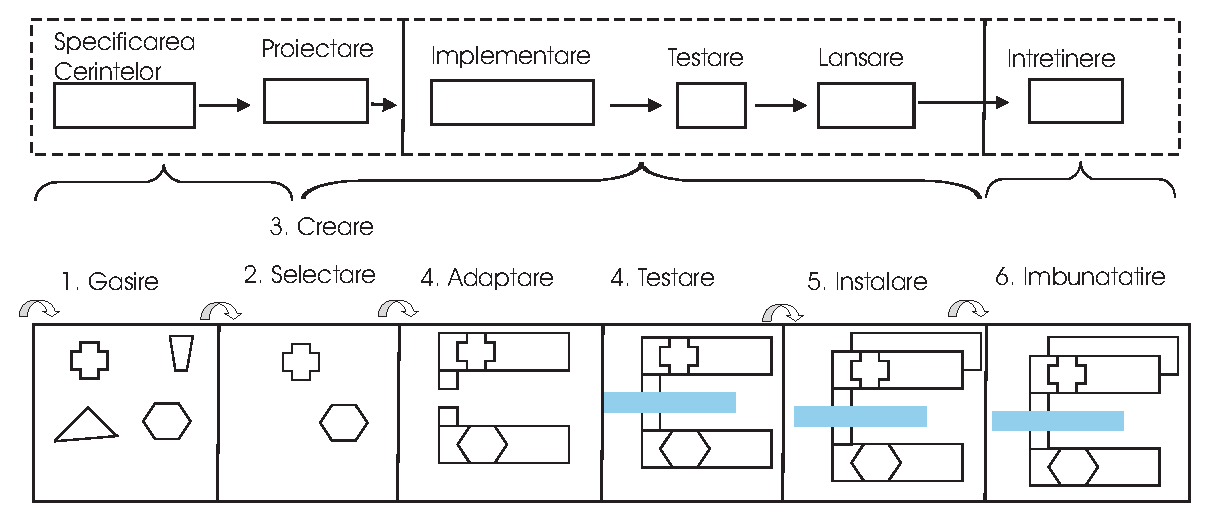
\includegraphics[scale=0.65]{./figures/fig_3_1.eps}
	\caption{Ciclul de dezvoltare al sistemelor bazate pe componente adaptat modelului cascadã}
	\label{FigCBSD}
\end{figure}

Inserarea și Referirea la Tabelul \ref{TabelSolutii}. 

\begin{table}[htbp]
\begin{center}
\begin{tabular}
{|p{120pt}|p{120pt}|p{120pt}|}
\hline
 Nume algoritm  &  Toate soluțiile &  Soluția optimã\\
\hline 
\hline Nume 1 & $20$ & $5$  \\
\hline Nume 2 & $20$ & $2$  \\
\hline
\end{tabular}
\end{center}
\caption{Soluții obținute }
\label{TabelSolutii}
\end{table}


Adaugarea și Referirea la o Ecuație \ref{LabelMyEquation}.


 \begin{equation}
     ws_N4 = w_{14}*N1 + W_{24}+N2 + w_{34}*N3
\label{LabelMyEquation}
 \end{equation}
